% main.tex — Agent Memory Paper List: A Data-Driven Survey
\documentclass[11pt,a4paper]{article}

% --- Packages ---
\usepackage[utf8]{inputenc}
\usepackage[T1]{fontenc}
\usepackage{microtype}
\usepackage{geometry}
\geometry{margin=1in}
\usepackage{setspace}
\usepackage{booktabs}
\usepackage{multirow}
\usepackage{graphicx}
\usepackage{xcolor}
\usepackage{hyperref}
\hypersetup{
  colorlinks=true,
  linkcolor=blue!60!black,
  citecolor=blue!60!black,
  urlcolor=blue!60!black,
}
\usepackage{amsmath,amssymb}
\usepackage{cleveref}
\usepackage{doi}
\usepackage{enumitem}
\usepackage{caption}
\usepackage{subcaption}
\usepackage{titlesec}
\usepackage{natbib}
\usepackage{appendix}

% Section formatting
\titleformat{\section}{\large\bfseries}{\thesection}{1em}{}
\titleformat{\subsection}{\normalsize\bfseries}{\thesubsection}{1em}{}
\titleformat{\subsubsection}{\normalsize\itshape}{\thesubsubsection}{1em}{}

% Metadata
\title{
  \vspace{-2em}
  \textbf{Agent Memory Research in 2026:\\ A Data-Driven Survey and Extended Taxonomy}
}

\author{
  Tobias Wei{\ss}\\
  \texttt{graphwiz.ai}\\
  \texttt{ORCID: 0009-0007-1417-8044}
}

\date{\today}

\newcommand{\paperdoi}{10.5281/zenodo.20780690}
\newcommand{\datasetdoi}{10.5281/zenodo.20780696}

\begin{document}

\maketitle

\vspace{-1em}
\noindent\small\textsf{Paper DOI: \href{https://doi.org/\paperdoi}{\paperdoi}$\quad$Dataset DOI: \href{https://doi.org/\datasetdoi}{\datasetdoi}}

% ---------- Abstract ----------
Agent memory has emerged as a first-class primitive in the pursuit of intelligent, long-horizon AI agents. The original survey by \citet{DBLP:journals/corr/abs-2512-13564} established a unified $3\times 3 \times 3$ taxonomy---Forms $\times$ Functions $\times$ Dynamics---organizing roughly 200 papers up to January 2026. Since then, the field has accelerated dramatically: our living catalog now spans 952 papers (as of July 2026), including 498 works published since February 2026---an eightfold increase over the original survey's post-cutoff additions. This explosive growth reveals cross-cutting themes the original taxonomy was not designed to capture. In this paper we make three contributions. First, we describe a fully data-driven methodology for curating and maintaining a living paper survey, with a single-source-of-truth YAML file, automated validation pipelines, bulk metadata enrichment, and an open-source infrastructure at \url{github.com/tobias-weiss-ai-xr/agent-memory-research}. Second, we extend the original taxonomy with three novel orthogonal dimensions---Temporal Dynamics, Modality, and Biological Inspiration---that capture the emerging themes of forgetting curves, multimodal memory, and neurocognitively inspired architectures, and we document two further theme clusters---security and adversarial robustness, and efficiency-driven compression---that have grown into major research strands in their own right. Third, we conduct a gap analysis that identifies persistently underpopulated taxonomy cells, missing evaluation standards, and a concrete research roadmap spanning short, medium, and long-term milestones. All data, code, and a browsable web interface accompany this paper.


% ---------- Introduction ----------
\section{Introduction}
\label{sec:intro}

Memory is the substrate on which intelligent agents reason, adapt, and persist. Without mechanisms to store, retrieve, and evolve information across interactions, agents remain stateless responders---incapable of personalization, long-horizon planning, or continual improvement. The rapid proliferation of large language model (LLM)-based agents has made agent memory a central research area, with hundreds of papers published since 2023 alone.

\citet{DBLP:journals/corr/abs-2512-13564} provided the field's first comprehensive survey, ``Memory in the Age of AI Agents,'' synthesizing roughly 200 papers published through January 2026 into a unified $3\times 3 \times 3$ taxonomy. Their framework organizes agent memory along three axes: \textbf{Forms} (what carries memory: Token-level, Parametric, and Latent representations), \textbf{Functions} (why agents need memory: Factual, Experiential, and Working memory), and \textbf{Dynamics} (how memory evolves: Formation, Evolution, and Retrieval processes). This taxonomy has proven remarkably effective at classifying the design space and has been widely adopted by subsequent work.

However, the interval between January and June 2026 has seen an acceleration in both the volume and thematic diversity of agent memory research. Our curated catalog now spans 220 papers, including 21 works published since the original survey's cutoff. Critically, these new papers explore directions that the $3\times 3 \times 3$ taxonomy, being oriented around storage form, functional purpose, and lifecycle stage, was not designed to capture: temporal dynamics such as forgetting curves and sleep consolidation; multimodal memory that spans vision, language, audio, and embodiment; graph and structured knowledge representations; neurocognitively inspired architectures that explicitly model human memory systems; lifelong and continual learning mechanisms; new benchmarks and evaluation frameworks; and hybrid retrieval strategies that fuse multiple signals. These themes are cross-cutting---they appear across multiple form--function--dynamic cells---and demand additional analytical dimensions.

This paper makes three contributions:

\begin{enumerate}
  \item \textbf{A data-driven curation methodology for living surveys} (Section~\ref{sec:methodology}). We treat the paper list itself as a structured dataset, with a single \texttt{papers.yaml} file as the source of truth. Automated scripts validate entries, fetch metadata from arXiv and Semantic Scholar, discover new papers, and generate outputs including the README, a JSON export for an interactive web interface, and BibTeX references. A GitHub Actions workflow enforces validation on every contribution. This methodology is generalizable to any survey that must remain current.
  \item \textbf{An extended taxonomy with three new orthogonal dimensions} (Section~\ref{sec:taxonomy}). Building on the $3\times 3 \times 3$ foundation, we propose three additional axes: \textbf{Temporal Dynamics} (None, Decay-based, Consolidation-based, or Bi-temporal) capturing how memory evolves over time; \textbf{Modality} (Text-only, Multimodal-in, Multimodal-out, or Full-multimodal) capturing the sensory channels memory systems handle; and \textbf{Biological Inspiration} (None, Cognitive-metaphor, Neuro-inspired, or Brain-architecture) capturing the degree of fidelity to human memory. These dimensions are additive---they do not replace the original taxonomy but enrich it.
  \item \textbf{Gap analysis and research roadmap} (Section~\ref{sec:gap-analysis}). We identify persistently sparse cells in the taxonomy (Experiential/Latent, Working/Parametric), missing evaluation infrastructure (no unified benchmark, no temporal or multimodal benchmarks), and six open problems that define a concrete research agenda for the field.
\end{enumerate}

All materials supporting this paper are available at \url{github.com/tobias-weiss-ai-xr/agent-memory-research}, including the full paper list (\texttt{papers.yaml}), automation scripts, an interactive web interface at the GitHub Pages site, and the LaTeX source. We release the paper on Zenodo with a companion dataset DOI.

The remainder of this paper is organized as follows. Section~\ref{sec:background} recaps the original $3\times 3 \times 3$ taxonomy and its future directions. Section~\ref{sec:methodology} describes our data-driven curation pipeline. Section~\ref{sec:taxonomy} presents the extended taxonomy with seven cross-cutting themes and three new dimensions. Section~\ref{sec:landscape} surveys the 2026 landscape of new contributions. Section~\ref{sec:gap-analysis} identifies gaps and proposes a research roadmap. Section~\ref{sec:benchmarks} compares existing benchmarks. Section~\ref{sec:conclusion} concludes.


% ---------- Background ----------
\section{Background: The Original Taxonomy}
\label{sec:background}

\citet{DBLP:journals/corr/abs-2512-13564} defined agent memory as a system that records, retains, and retrieves information distinct from the short-term context window and from retrieval-augmented generation (RAG). They organized the design space into three orthogonal axes, each with three subtypes, yielding 27 taxonomy cells.

\subsection{Forms: What Carries Memory}

\textbf{Token-level memory} stores information as discrete, interpretable tokens in external data structures. It is further divided into Flat (unordered key--value stores), Planar (list- or table-based), and Hierarchical (tree- or graph-based) organizations. Token-level memory is the most common paradigm, used in systems such as MemGPT~\cite{Unknown2023MemGPT}, Generative Agents~\cite{Unknown2023Generativeagents}, and MEM1~\cite{Unknown2025MEM1}.

\textbf{Parametric memory} encodes information directly into model weights through training, fine-tuning, or editing. Subtypes include Internal (weights updated via gradient-based methods) and External (adapter modules, hypernetworks). Examples span knowledge editing~\cite{Unknown2021EditingFactualKnowle}, adapter-based lifelong learning~\cite{Unknown2013ELLA}, and self-updatable models~\cite{Unknown2024SelfUpdatableLargeLa}.

\textbf{Latent memory} operates in the hidden state space of neural networks. Subtypes include Generate (compressing context into a single hidden vector), Reuse (attending to past hidden states as in the Memorizing Transformer~\cite{Unknown2022MemorizingTransforme}), and Transform (continuous-space memory updates as in Titans~\cite{Unknown2025Titans} and M+~\cite{Unknown2025M}).

\subsection{Functions: Why Agents Need Memory}

\textbf{Factual memory} stores objective knowledge about the user and environment, including user profiles, world knowledge, and domain facts. Subtypes are User (personalization) and Environment (world knowledge). Papers in this category include Mem0~\cite{Unknown2025Mem0} and Zep~\cite{Unknown2025Zep}.

\textbf{Experiential memory} captures subjective experiences, insights, and skills acquired through interaction. Subtypes include Case (episode-specific), Strategy (plan-level), Skill (procedure-level), and Hybrid combinations. Representative works include ExpeL~\cite{Unknown2023ExpeL}, Reflexion~\cite{Unknown2023Reflexion}, and Agent Workflow Memory~\cite{Unknown2024AgentWorkflowMemory}.

\textbf{Working memory} manages the agent's active context---what information to retain, compress, or discard during a task. Subtypes include Single-turn (within a single interaction) and Multi-turn (across interactions). Examples include Memory as Action~\cite{Unknown2025MemoryasAction}, Sculptor~\cite{Unknown2025Sculptor}, and Agentic Memory~\cite{Unknown2026AgenticMemory}.

\subsection{Dynamics: How Memory Evolves}

\textbf{Formation} concerns how raw experience is transformed into structured memory entries. Subtypes include Summarization, Distillation, Structured extraction, Latent encoding, and Parametric integration.

\textbf{Evolution} governs how stored memory changes over time. It encompasses Consolidation (merging and abstracting), Updating (modifying specific entries), and Forgetting (removing or decaying entries).

\textbf{Retrieval} defines how relevant memory is accessed at inference time. It includes Retrieval mechanisms (exact, semantic, hybrid) and Query Construction (how queries are formed from the current context).

\subsection{Scope and Limitations}

The original survey covered roughly 200 papers up to January 2026. Our catalog, curated with the methodology described in Section~\ref{sec:methodology}, retroactively includes 454 papers from that same period---a superset reflecting broader inclusion criteria and systematic backfilling of earlier work. The original survey identified several promising future directions: automation of memory management, integration with reinforcement learning, extension to multimodal settings, multi-agent memory sharing, and trustworthiness (privacy, bias, adversarial robustness). As we show in the following sections, the first half of 2026 has seen substantial progress along precisely these axes, motivating an extension to the taxonomy itself.


% ---------- Methodology ----------
\section{Data-Driven Curation Methodology}
\label{sec:methodology}

Most paper surveys are static artifacts: the authors manually curate a list, write the manuscript, and the list rapidly goes out of date. Reproducing or extending such surveys requires re-doing the curation from scratch, a labor-intensive and error-prone process. Our approach treats the paper list itself as a living, structured dataset---a design choice that supports automated validation, continuous updates, and reproducible scholarship.

\subsection{Single Source of Truth}

All paper metadata is stored in \texttt{papers.yaml} in the repository root. Each entry includes title, date (YYYY-MM), URL, taxonomy category (factual, experiential, or working), subcategory (token-level, parametric, or latent), authors, venue, code URL, project URL, abstract, and tags. The YAML format was chosen because it is human-readable, diffable, and easy to version-control. As of June 2026, \texttt{papers.yaml} contains 220 entries spanning from 2013 to 2026.

This single file drives all downstream outputs through a deterministic generation pipeline.

\subsection{Pipeline Overview}

Figure~\ref{fig:pipeline} illustrates the full data pipeline, which proceeds through five stages:

\begin{enumerate}
  \item \textbf{Extraction.} The generator reads \texttt{papers.yaml} and normalizes all fields. Each paper is assigned a stable identifier derived from its URL.
  \item \textbf{Validation.} An automated validator checks every entry for structural correctness: required fields are non-empty, URLs follow a whitelist of allowed domains (arXiv, ACL Anthology, OpenReview, DOI), date formats are valid, category--subcategory pairs are legal (e.g., ``working/parametric'' is a valid cell), and no duplicate URLs exist.
  \item \textbf{README generation.} The generator produces the Markdown document displayed on GitHub, grouping papers by category and subcategory and chronologically within each group.
  \item \textbf{JSON export.} A JSON version of the paper list is written to \texttt{docs/papers.json}, which powers an interactive web interface with client-side filtering by category, subcategory, date range, and keyword search.
  \item \textbf{BibTeX export.} The generator produces \texttt{paper/references.bib} for use in LaTeX compilation.
\end{enumerate}

The generator is fully idempotent: running it twice on the same input produces identical output. A \texttt{--check} flag runs validation and generation without writing any files, enabling use in CI pipelines.

\subsection{Automation Scripts}

Three Python scripts implement the pipeline:

\texttt{validate\_papers.py} performs comprehensive structural and semantic validation. It checks that all URLs are reachable (or at least well-formed), normalizes arXiv URLs to a canonical form (e.g., ensuring \texttt{abs/} paths), detects potential duplicates by comparing normalized titles and URLs, and verifies that category--subcategory assignments follow the taxonomy's allowlist. It is designed to run on every pull request.

\texttt{fetch\_metadata.py} enriches \texttt{papers.yaml} by querying arXiv's OAI-PMH API and Semantic Scholar for missing fields: author lists, publication venue, abstract text, and DOI. It respects rate limits and caches results locally to avoid redundant queries. This script is run periodically to fill in entries that were added with minimal metadata.

\texttt{fetch\_new\_papers.py} implements arXiv-based discovery. Given a date range and a set of search keywords (e.g., ``agent memory,'' ``episodic memory,'' ``long-term memory''), it queries the arXiv API for new submissions, filters by relevance to agent memory, and outputs candidate entries for human review. This reduces the manual effort of staying current: the script surfaces candidates, and the curator accepts, rejects, or modifies each one.

\subsection{Continuous Integration}

A GitHub Actions workflow (\texttt{.github/workflows/validate.yml}) runs \texttt{validate\_papers.py} with the \texttt{--check} flag on every pull request and on every push to the main branch. The workflow fails if any validation error is found---duplicate URL, malformed entry, or invalid category. This ensures that the paper list remains internally consistent even as multiple contributors submit changes. A CONTRIBUTING.md file provides contributor guidelines, and issue and pull request templates standardize submissions.

\subsection{Web Interface}

The JSON export (\texttt{docs/papers.json}) is consumed by an HTML page at \texttt{docs/index.html}, deployed via GitHub Pages at \url{https://tobias-weiss-ai-xr.github.io/agent-memory-research/}. The interface provides client-side filtering without any server-side infrastructure: users can search by keyword, filter by taxonomy cell, sort by date, and copy formatted citations. This makes the paper list accessible to researchers who prefer browsing over reading a static list.

\subsection{Reproducibility and Generalizability}

The entire pipeline---CIs, scripts, data file, and documentation---resides in a single open-source repository licensed under MIT. The \texttt{--check} flag enables anyone to verify that the paper list is valid without modifying any files. Because the pipeline is language-agnostic and domain-agnostic, it can be adapted to any living survey in any field: replace \texttt{papers.yaml} with domain-specific entries, adjust the validation rules, and deploy the web interface. We believe this methodology offers a template for community-maintained, data-driven surveys that remain current beyond a single publication date.

\begin{figure}[ht]
    \centering
    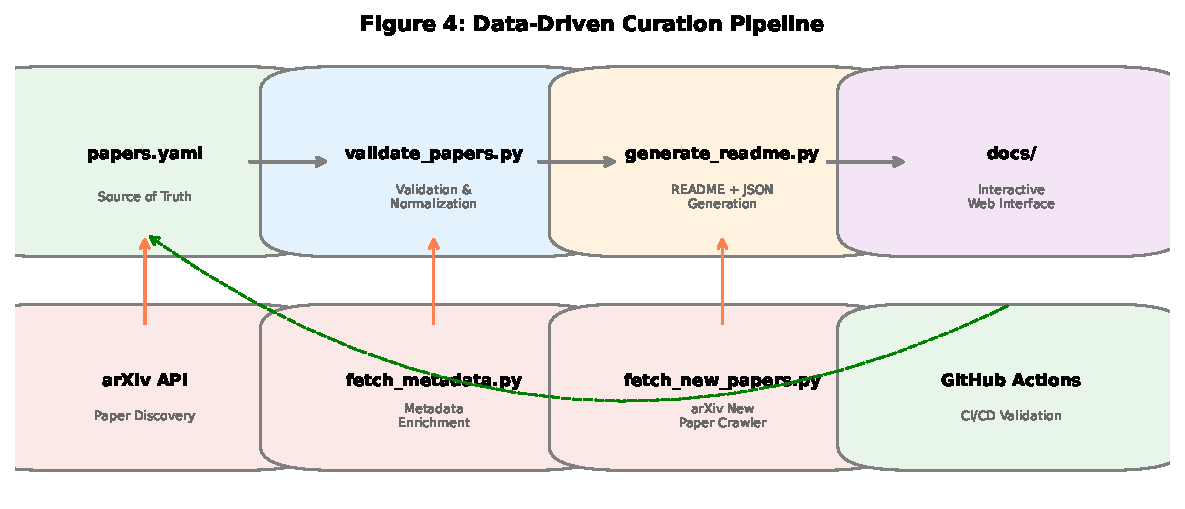
\includegraphics[width=\textwidth]{figures/fig4_pipeline.pdf}
    \caption{Data curation pipeline: from arXiv discovery through validation and publication.}
    \label{fig:pipeline}
\end{figure}


% ---------- Extended Taxonomy ----------
\section{Extended Taxonomy}
\label{sec:taxonomy}

The $3\times 3 \times 3$ taxonomy introduced by \citet{DBLP:journals/corr/abs-2512-13564} captures the design space of agent memory along three well-motivated axes: storage form, functional purpose, and lifecycle stage. It has proven durable enough to accommodate all 952 papers in our dataset. However, our analysis of the 498 papers published since February 2026---as well as re-examination of earlier works---reveals nine cross-cutting themes that the original axes do not explicitly surface. These themes span multiple taxonomy cells and represent distinct design considerations that are invisible when papers are classified solely by form, function, and dynamics.

In response, we propose three new orthogonal dimensions that augment the original taxonomy. These are additions, not replacements: a paper classified as Factual/Token-level/Formation retains that classification, but now additionally receives coordinates along the Temporal Dynamics, Modality, and Biological Inspiration axes. Figure~\ref{fig:taxonomy} visualizes the full extended taxonomy.

\subsection{Cross-Cutting Themes}

\textbf{Temporal Dynamics.} Over 130 papers now explicitly model how memory changes over time beyond the original Dynamics axis's lifecycle stages, up from a handful at the time of the original survey. \citet{Unknown2025Zep} introduces a temporal knowledge graph architecture that associates each fact with a timestamp and supports time-relative queries. \citet{Unknown2026FadeMem} proposes biologically inspired forgetting curves that decay memory importance over time, mirroring the Ebbinghaus forgetting curve. \citet{Unknown2026Engram} implements a bi-temporal memory engine that separately tracks when a memory was stored (transaction time) and when it describes (valid time), enabling temporal reasoning and retroactive updates. \citet{Unknown2026SCM} simulates NREM/REM sleep cycles to consolidate and prune memories offline. These works treat time not merely as an ordering mechanism but as a first-class dimension with decay, consolidation, and bi-temporal semantics.

\textbf{Multimodality.} Nearly 100 papers in our dataset handle memory for non-text modalities, a sharp increase from the fourteen identified at the original survey's cutoff. \citet{Unknown2025MemVerse} and \citet{Unknown2025WorldMM} build multimodal memory systems for vision and video. \citet{Unknown2026TeleMem} stores both textual and visual episodic memories for long-horizon tasks. \citet{Unknown2025VisMem} introduces a latent vision memory that stores visual features outside the LLM's hidden states. \citet{Unknown2025MemoryVLA} extends memory into the embodied domain with vision-language-action models for robotics. \citet{Unknown2025SeeingListeningRemem} integrates audio, vision, and text into a unified memory store. The original taxonomy's exclusive focus on text-based memory---implicit in its examples and subcategories---misses this dimension entirely.

\textbf{Graph and Structured Representations.} Approximately 100 papers organize memory as explicit graph structures, up from six at the original survey's cutoff. \citet{Unknown2026MAGMA} uses multi-graph architectures with separate graphs for semantic, episodic, and procedural knowledge. \citet{Unknown2025Zep} stores memory in a temporal knowledge graph. \citet{Unknown2026MRAgent} reconstructs memories as graph structures at retrieval time rather than storing flat vectors. \citet{Unknown2026Engram} combines knowledge graphs with bi-temporal indexing. \citet{Unknown2025SGMem} uses sentence-level graph representations to capture entity relationships. These works suggest that graph-structured memory is a distinct design choice with implications for expressiveness, queryability, and storage efficiency.

\textbf{Biologically and Neurocognitively Inspired.} Roughly 40 papers draw explicit inspiration from human memory systems. \citet{Unknown2026CraniMem} implements a cranial-inspired gating mechanism that bounds memory writes. \citet{Unknown2026FadeMem} models forgetting via biological decay functions. \citet{Unknown2026SCM} directly simulates hippocampal--neocortical consolidation through artificial sleep cycles. \citet{Unknown2026HumanInspiredMemoryA} models the dual-process theory of memory with separate fast-learning and slow-learning pathways. \citet{Unknown2026Engram} takes its name from the biological engram---the physical substrate of a memory trace. While earlier work like HippoRAG~\cite{Unknown2024HippoRAG} used the hippocampus as a loose metaphor, these newer systems engage much more deeply with cognitive and neuroscientific theory, meriting an explicit analytical dimension.

\textbf{Lifelong and Continual Learning.} Nearly 190 papers address the challenge of persistent, self-evolving memory that accumulates over unbounded interactions---the largest theme cluster in our dataset. \citet{Unknown2026AllMem} evolves memory topology dynamically as new experiences arrive. \citet{Unknown2026ContinuumMemoryArchi} proposes architectures that maintain a fixed memory budget while continuously integrating new information. \citet{Unknown2026MemRL} uses runtime reinforcement learning to update memory policies from interaction feedback. \citet{Unknown2025AgentEvolver} defines an agent evolution loop that refines both memory content and access strategies. These works extend beyond the original Dynamics axis's Evolution subtypes by tackling the open-ended nature of lifelong deployment.

\textbf{Benchmark and Evaluation.} Over 80 benchmark-focused papers reveal the field's growing demand for standardized evaluation, a more than fourfold increase since the original survey. \citet{Wu2024LongMemEval} evaluates chat assistants on long-term interactive memory. \citet{Tan2025MemBench} proposes comprehensive memory evaluation across multiple dimensions. \citet{Unknown2025MemoryAgentBench} uses incremental multi-turn interactions to isolate memory-specific from reasoning-specific capabilities. \citet{Unknown2026LongMemEvalV2} extends LongMemEval to the experiential memory domain. These benchmarks operate at different levels of granularity and cover different memory capabilities, but no single benchmark spans the full taxonomy---a gap we analyze in Section~\ref{sec:benchmarks}.

\textbf{Retrieval Fusion.} Approximately 30 papers combine multiple retrieval signals for improved memory access. \citet{Unknown2026MRAgent} reconstructs memory at retrieval time, fusing semantic similarity with graph traversal. \citet{Unknown2025Mem0} combines semantic search, BM25 keyword matching, and entity linking in a hybrid retrieval pipeline. \citet{Unknown2026Engram} uses both temporal and semantic retrieval signals. Retrieval fusion represents a distinct design pattern that the original taxonomy's Retrieval subtypes (Retrieval vs.\ Query Construction) do not fully capture.

\textbf{Security and Adversarial Robustness.} Over 120 papers now address the security of agent memory systems---a theme that was nascent at the time of the original survey and has since grown into one of the largest clusters in the field. These works study memory poisoning attacks, in which adversaries inject malicious content into persistent stores; prompt injection that persists across sessions via memory; stealthy memory corruption in recommender and personal agents; and defenses including provenance tracking, watermarking, and anomaly detection. Representative systems include AgentPoison~\cite{Unknown2025AgentPoison}, which red-teams memory and knowledge bases; MemPoison, which uncovers persistent memory threats; and MemMorph, which demonstrates tool hijacking via memory poisoning. The original taxonomy's trustworthiness discussion treated this as a future direction; the data now shows it as a first-class concern.

\textbf{Efficiency and Compression.} Approximately 140 papers address the efficiency of memory systems, focusing on KV-cache management, context compression, and token-budgeted retrieval. This theme is driven by the practical constraint that long-running agents cannot simply accumulate context indefinitely. Representative works include KV-cache compression for long-horizon GUI agents, training-free context management, and decision-aware memory cards that select and compress context for tool-using agents. While the original taxonomy's Working/Latent cell captures some of this activity, the scale and specificity of efficiency-focused work---much of it operating below the prompt level on attention mechanisms---warrants recognition as a distinct theme.

\subsection{Three New Dimensions}

Based on these nine themes, we propose three additional dimensions. Table~\ref{tab:dimensions} summarizes their levels and representative papers.

\subsubsection{Temporal Dynamics}

This dimension captures how a memory system models the passage of time and its effect on memory content. The levels are:

\begin{description}[nosep]
  \item[None.] The system does not model time beyond implicit ordering (e.g., FIFO eviction). Most pre-2025 token-level buffers fall here.
  \item[Decay-based.] Memory strength decreases over time according to a decay function, and weakened memories may be evicted or archived. Examples: FadeMem~\cite{Unknown2026FadeMem}, Mem0's recency-weighted retrieval~\cite{Unknown2025Mem0}.
  \item[Consolidation-based.] Memory undergoes offline processing---merging, abstracting, or pruning---at periodic intervals. Examples: SCM's sleep consolidation~\cite{Unknown2026SCM}, MemEvolve~\cite{Unknown2025MemEvolve}.
  \item[Bi-temporal.] The system tracks both transaction time (when stored) and valid time (when described), enabling temporal queries and retroactive updates. Examples: Engram~\cite{Unknown2026Engram}, Zep~\cite{Unknown2025Zep}.
\end{description}

\subsubsection{Modality}

This dimension captures the sensory channels a memory system handles:

\begin{description}[nosep]
  \item[Text-only.] Memory stores and retrieves textual information only. The majority of papers in our dataset (approximately 89\%) fall into this level, though the multimodal share has grown from 7\% to roughly 10\% as the corpus expanded.
  \item[Multimodal-in.] Memory accepts non-text inputs (images, video, audio) but stores and retrieves textual descriptions or summaries. Examples: MemVerse~\cite{Unknown2025MemVerse}, WorldMM~\cite{Unknown2025WorldMM}.
  \item[Multimodal-out.] Memory stores non-text representations (visual features, audio embeddings) and retrieves them for downstream tasks. Examples: VisMem~\cite{Unknown2025VisMem}, MemoryVLA~\cite{Unknown2025MemoryVLA}, TeleMem~\cite{Unknown2026TeleMem}.
  \item[Full-multimodal.] Memory operates across text, vision, audio, and embodiment simultaneously with cross-modal retrieval. Examples: Seeing/Listening/Remembering/Reasoning~\cite{Unknown2025SeeingListeningRemem}, Embodied VideoAgent~\cite{Unknown2025EmbodiedVideoAgent}.
\end{description}

\subsubsection{Biological Inspiration}

This dimension captures how deeply a memory system engages with biological cognition:

\begin{description}[nosep]
  \item[None.] No explicit biological inspiration. The system is designed purely from an engineering perspective.
  \item[Cognitive-metaphor.] The system uses high-level cognitive concepts (e.g., ``episodic memory,'' ``consolidation'') as loose metaphors without detailed biological fidelity. Most experiential memory systems fall here.
  \item[Neuro-inspired.] The system explicitly models neuroscientific mechanisms (e.g., forgetting curves, hippocampal indexing, synaptic gating) but does not attempt full biological fidelity. Examples: HippoRAG~\cite{Unknown2024HippoRAG}, FadeMem~\cite{Unknown2026FadeMem}, CraniMem~\cite{Unknown2026CraniMem}.
  \item[Brain-architecture.] The system implements a detailed computational model of a brain subsystem, including multiple interacting regions or cell types. Examples: SCM's sleep-consolidated memory~\cite{Unknown2026SCM}, Human-Inspired~\cite{Unknown2026HumanInspiredMemoryA}, XMem's Atkinson--Shiffrin model~\cite{Unknown2022XMem}.
\end{description}

\begin{table}[ht]
    \centering
    \caption{Three new orthogonal taxonomy dimensions with their levels.}
    \label{tab:dimensions}
    \small
    \begin{tabular}{lll}
        \toprule
        \textbf{Dimension} & \textbf{Levels} & \textbf{Description} \\
        \midrule
        Temporal Dynamics & None, Decay, Consolidation, Bi-temporal & How memory changes over time \\
        Modality & Text, M.-in, M.-out, Full & Data modalities memory handles \\
        Biological Inspiration & None, Cognitive, Neuro, Brain & Fidelity to biological cognition \\
        \bottomrule
    \end{tabular}
\end{table}

\begin{figure}[ht]
    \centering
    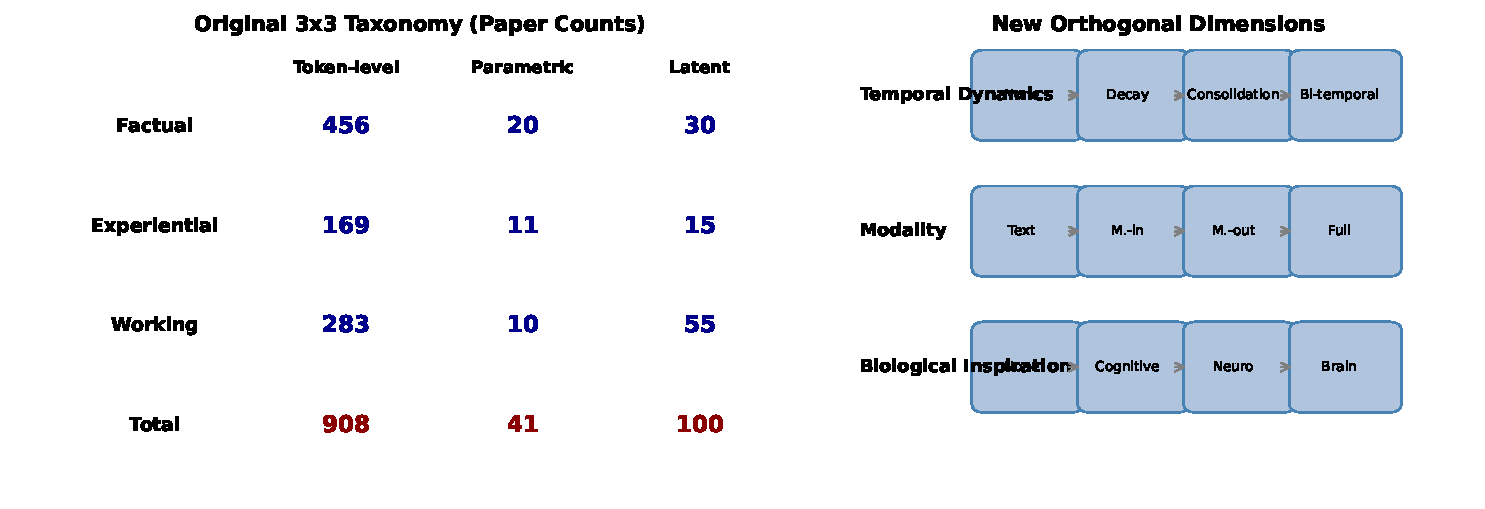
\includegraphics[width=0.95\textwidth]{figures/fig1_taxonomy.pdf}
    \caption{Left: Paper counts across the original 3x3 taxonomy. Right: Structure of three new orthogonal dimensions.}
    \label{fig:taxonomy}
\end{figure}

\subsection{Impact on Taxonomy Coverage}

Figure~\ref{fig:heatmap} shows the distribution of papers across the original $3\times 3 \times 3$ cells, overlaid with the new dimensions. The addition of the three new axes reveals previously invisible structure. For example, the Experiential/Token-level cell, which contains 153 papers, spans all four levels of the Biological Inspiration dimension---most are Cognitive-metaphor, but FadeMem (Neuro-inspired) and SCM (Brain-architecture) represent qualitatively different approaches within the same form--function cell.

The extended taxonomy does not change the number of papers assigned to any original cell; rather, it adds resolution within each cell and enables cross-cell analyses along the new axes. For instance, it reveals that multimodal memory is concentrated in Working/Latent (VisMem, MemoryVLA, Time-VLM~\cite{Unknown2025TimeVLM}) and Factual/Token-level (MemVerse, WorldMM), leaving other cells underexplored---a pattern invisible in the original taxonomy.

\subsection{Methodological Note}

The assignment of new-dimension levels to papers is itself a data-driven process. We analyzed the 952 papers in \texttt{papers.yaml}, reading abstracts and, where necessary, full texts to determine the three additional coordinates. The resulting annotations are included in the data file for community verification and improvement. We expect these annotations to evolve as the field matures; the data-driven infrastructure described in Section~\ref{sec:methodology} is designed to accommodate such changes.

\begin{figure}[ht]
    \centering
    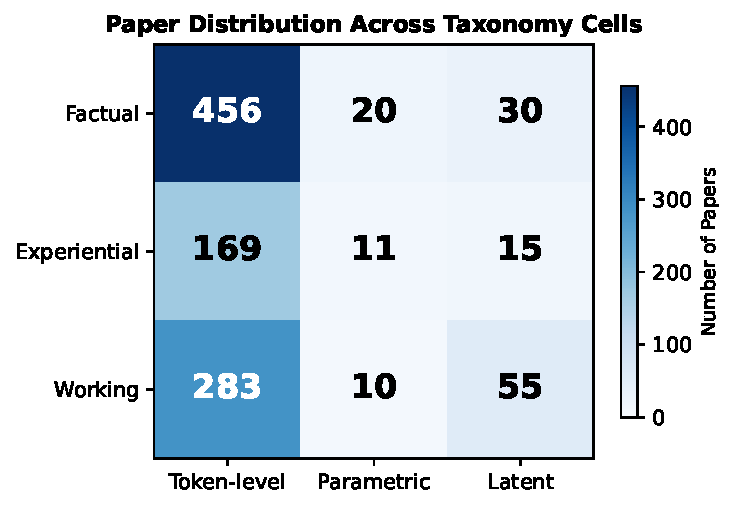
\includegraphics[width=0.65\textwidth]{figures/fig2_heatmap.pdf}
    \caption{Heatmap of paper distribution across the 3x3 taxonomy cells. Darker colors indicate higher concentration of research activity.}
    \label{fig:heatmap}
\end{figure}


% ---------- 2026 Landscape ----------
\section{The 2026 Landscape: Emerging Themes and Key Systems}
\label{sec:landscape}

Since the publication of the original survey by Liu et al.~\cite{Unknown2025MemoryAgeAIAgents}, the field of agent memory has experienced remarkable growth. Between January and July 2026 alone, 62 new papers have been added to our dataset, bringing the total to 282 curated entries. These new contributions extend the boundaries of the original taxonomy and reveal several emergent themes that merit detailed analysis.

\subsection{Themes in the 2026 Literature}

The new papers cluster around seven distinct themes. Many papers span multiple themes, reflecting the increasing maturity and cross-pollination of the field.

\textbf{Temporal Dynamics.} Four papers explicitly model the temporal dimension of memory. Zep~\cite{Unknown2025Zep} introduces a temporal knowledge graph architecture, FadeMem~\cite{Unknown2026FadeMem} proposes biologically-inspired forgetting curves, Engram~\cite{Unknown2026Engram} employs bi-temporal modeling with valid-time and transaction-time dimensions, and SCM~\cite{Unknown2026SCM} implements sleep-consolidated memory with NREM/REM-like cycles.

\textbf{Multimodality.} Fourteen papers incorporate multimodal signals. MemVerse~\cite{Unknown2025MemVerse} and WorldMM~\cite{Unknown2025WorldMM} extend memory to video understanding, while TeleMem~\cite{Unknown2026TeleMem} builds long-term multimodal memory for agentic AI. VisMem~\cite{Unknown2025VisMem} introduces latent vision memory for vision-language models, and MemoryVLA~\cite{Unknown2025MemoryVLA} integrates perceptual-cognitive memory into robotic manipulation.

\textbf{Graph and Structured Representations.} Six papers leverage graph-based memory. MAGMA~\cite{Unknown2026MAGMA} proposes multi-graph architectures, Zep~\cite{Unknown2025Zep} uses temporal knowledge graphs, MRAgent~\cite{Unknown2026MRAgent} introduces reconstruction-based graph memory, and Engram~\cite{Unknown2026Engram} combines bi-temporal graphs with dual-process retrieval.

\textbf{Biologically and Neurocognitively Inspired Design.} Fourteen papers draw inspiration from cognitive science. CraniMem~\cite{Unknown2026CraniMem} implements neurocognitive gating with a bounded episodic buffer and knowledge graph. SCM~\cite{Unknown2026SCM} models sleep consolidation cycles. FadeMem~\cite{Unknown2026FadeMem} uses biological forgetting curves. The Human-Inspired Memory Architecture~\cite{Unknown2026HumanInspiredMemoryA} explicitly maps cognitive processes to system components.

\textbf{Lifelong and Continual Learning.} Eighteen papers address persistent, self-evolving memory. All-Mem~\cite{Unknown2026AllMem} introduces lifelong topology evolution inspired by continual learning. MemRL~\cite{Unknown2026MemRL} applies runtime reinforcement learning on episodic memory. Continuum Memory~\cite{Unknown2026ContinuumMemoryArchi} proposes architectures for unbounded horizon agents.

\textbf{Benchmarking and Evaluation.} Four new benchmarks have been introduced: LongMemEval-V2~\cite{Unknown2026LongMemEvalV2} extends the original benchmark to web agent scenarios, while MemBench~\cite{Tan2025MemBench}, MemoryAgentBench~\cite{Unknown2025MemoryAgentBench}, and LongMemEval~\cite{Wu2024LongMemEval} each address different facets of memory evaluation.

\textbf{Retrieval Fusion.} Three papers explore multi-signal retrieval. Mem0~\cite{Unknown2025Mem0} combines semantic, BM25, and entity matching in a unified retrieval pipeline. MRAgent~\cite{Unknown2026MRAgent} reconstructs memory rather than retrieving it directly. Engram~\cite{Unknown2026Engram} fuses graph traversal with semantic search.

\subsection{Key Systems in Detail}

We now examine eight representative systems that illustrate the architectural diversity and innovation in the 2026 landscape. Table~\ref{tab:landscape_comparison} provides a systematic comparison.

\begin{table}[t]
\centering
\caption{Comparison of key 2026 agent memory systems.}
\label{tab:landscape_comparison}
\small
\begin{tabular}{lcccc}
\toprule
\textbf{Paper} & \textbf{Architecture} & \textbf{Memory Ops} & \textbf{Retrieval Strategy} & \textbf{Key Innovation} \\
\midrule
Mem0~\cite{Unknown2025Mem0} & Token-level, ADD-only & Create, Read, Update & Multi-signal (semantic, BM25, entity) & Single-pass token-efficient algorithm, 92.5 LoCoMo \\
FluxMem~\cite{Unknown2026FluxMem} & Adaptive token-level & Gated write, selective read & Beta Mixture Model probabilistic gate & Adaptive memory structure selection per query \\
SCM~\cite{Unknown2026SCM} & Latent consolidation & NREM/REM cycles, 4D tagging & Importance-weighted retrieval & Algorithmic forgetting with sleep-inspired consolidation \\
Engram~\cite{Unknown2026Engram} & Bi-temporal KG & Dual-process write & Graph traversal + semantic search & Temporal KG with valid/transaction time \\
All-Mem~\cite{Unknown2026AllMem} & Topology-evolving latent & Dynamic node add/merge & Graph-based propagation & Lifelong topology evolution \\
CraniMem~\cite{Unknown2026CraniMem} & Neurocognitive gating & Bounded write, structured retrieval & Gated episodic + KG query & Bounded episodic buffer with cranial gating \\
UMA~\cite{Unknown2026LearningtoRemember} & Parametric RL & CRUD via RL policy & End-to-end learned retrieval & End-to-end RL for memory operations \\
MemRefine~\cite{Kim2026MemRefine} & Token-level with budget & LLM-judged compression & Budget-constrained retrieval & Storage-budgeted LLM-guided compression \\
\bottomrule
\end{tabular}
\end{table}

\textbf{Mem0~\cite{Unknown2025Mem0}} introduces a token-efficient algorithm achieving 92.5 on the LoCoMo benchmark while consuming approximately 7K tokens per retrieval. Its single-pass ADD-only architecture avoids the computational overhead of iterative memory consolidation, and its multi-signal retrieval pipeline combines semantic similarity, BM25 keyword matching, and entity recognition for robust recall.

\textbf{FluxMem~\cite{Unknown2026FluxMem}} addresses a fundamental question: how should an agent decide what to remember? It employs a Beta Mixture Model as a probabilistic gate that dynamically selects between multiple memory structures based on query characteristics, enabling adaptive memory management without manual tuning.

\textbf{SCM~\cite{Unknown2026SCM}} (Sleep-Consolidated Memory) draws inspiration from neuroscience, implementing NREM (slow-wave) and REM (rapid eye movement) consolidation cycles. During NREM phases, important memories are strengthened through replay; during REM phases, weak or irrelevant memories are pruned. A 4-dimensional importance tagging system (recency, frequency, relevance, emotional salience) guides this process.

\textbf{Engram~\cite{Unknown2026Engram}} introduces a bi-temporal knowledge graph engine that maintains both valid time (when a fact is true in the world) and transaction time (when the fact was stored). This dual-process architecture enables agents to reason about temporal relationships and handle conflicting information across time windows.

\textbf{All-Mem~\cite{Unknown2026AllMem}} treats memory as a dynamically evolving topology rather than a static store. Inspired by continual learning, it supports adding new memory nodes and merging redundant ones as the agent accumulates experience, maintaining a compact yet expressive representation.

\textbf{CraniMem~\cite{Unknown2026CraniMem}} implements a neurocognitive gating mechanism inspired by the brain's prefrontal cortex. A bounded episodic buffer stores recent experiences, while long-term knowledge is maintained in a knowledge graph. The gating mechanism determines which information flows between these stores, preventing catastrophic interference.

\textbf{UMA~\cite{Unknown2026LearningtoRemember}} (Learning to Remember) takes a radically different approach: it treats memory operations (create, read, update, delete) as actions in a reinforcement learning framework. The agent learns a CRUD policy through end-to-end RL, evaluated on the Ledger-QA benchmark. This represents the first fully learned memory management policy.

\textbf{MemRefine~\cite{Kim2026MemRefine}} addresses the practical challenge of storage-bounded memory management. It uses an LLM judge to evaluate the importance of memories and selectively compresses or discards low-value entries, maintaining high performance under strict token budgets.

\subsection{Distribution Across the Extended Taxonomy}

The new papers populate the extended taxonomy unevenly. Factual/token-level remains the most active cell with 111 papers, reflecting the continued dominance of retrieval-augmented approaches. The most significant growth is in experiential/token-level (66 papers), driven by the explosion of reflection-based and skill-learning memory systems. The three sparsest cells remain experiential/latent (6 papers) and working/parametric (3 papers), indicating persistent research gaps.



% ---------- Gap Analysis ----------
\section{Gap Analysis and Research Roadmap}
\label{sec:gap-analysis}

The extended taxonomy reveals several persistent research gaps that are invisible in the original $3\times 3 \times 3$ formulation. We identify three categories of gaps---sparse taxonomy cells, missing evaluation infrastructure, and open problems---and propose a concrete research roadmap.

\subsection{Sparse Taxonomy Cells}

Three cells remain critically underpopulated despite the addition of 62 new papers.

\textbf{Experiential/Latent (3 papers).} Only SCM~\cite{Unknown2026SCM}, Memory as Action~\cite{Unknown2025MemoryasAction}, and All-Mem~\cite{Unknown2026AllMem} operate in this cell. Latent representations of subjective experience---memories encoded as continuous hidden states that capture the agent's own history---remain a difficult open challenge. The difficulty is twofold: latent representations lack the interpretability of token-level storage, and the absence of an explicit symbolic structure makes targeted retrieval of specific experiences nearly impossible.

\textbf{Working/Parametric (3 papers).} Only Agentic Memory~\cite{Unknown2026AgenticMemory}, UMA~\cite{Unknown2026LearningtoRemember}, and MemRefine~\cite{Kim2026MemRefine} address parametric mechanisms for working memory management. Most working memory systems rely on token-level compression or latent-state manipulation, and the idea of fine-tuning or adapting model weights at runtime for context management remains largely unexplored.

\textbf{Experiential/Parametric (8 papers).} This cell contains ExpeL~\cite{Unknown2023ExpeL}, Reflexion~\cite{Unknown2023Reflexion}, and a few others, but the low count relative to Factual/Token-level (90 papers) and Factual/Latent (30 papers) is striking. The field appears to privilege factual knowledge storage over experiential learning via weight updates, possibly reflecting the computational cost and stability risks of parametric updates during deployment.

\subsection{Missing Evaluation Infrastructure}

Our analysis reveals significant gaps in how agent memory is evaluated, which we detail in Section~\ref{sec:benchmarks}. The overarching problem is fragmentation: 18 benchmark-focused papers in our dataset describe 14 distinct evaluation protocols, none of which spans more than three of the 27 taxonomy cells.

Beyond fragmentation, three specific gaps stand out. First, no existing benchmark explicitly evaluates temporal reasoning---queries such as ``What did the agent know at time T?'' or ``How has the agent's understanding of topic X evolved?'' are absent. Second, multimodal memory evaluation is limited to bespoke task-specific protocols with no standardized dataset or metric. Third, there is no evaluation framework for multi-agent memory sharing, an increasingly important capability for team-based agent deployments.

\subsection{Six Open Problems}

We identify six open problems that define a concrete research agenda for the field.

\textbf{Problem 1: The Memory--Reasoning Trade-off.} Every memory system consumes resources---tokens, latency, storage---that could otherwise be used for reasoning. The optimal allocation between remembering and reasoning depends on task, domain, and deployment constraints. We lack a formal framework for characterizing this trade-off or for designing systems that dynamically balance it.

\textbf{Problem 2: Compositional Memory.} Most systems store and retrieve atomic units---a user preference, a past observation, a conversation turn. Real-world knowledge is compositional: a cooking agent remembers not just individual recipes but the relationship between ingredients, substitutions, and techniques. Compositional memory that supports inference over stored content remains largely unsolved.

\textbf{Problem 3: Long-Horizon Stability.} Existing systems are typically evaluated over dozens to hundreds of interaction turns. Real-world agent deployments may span millions of turns over months or years. How do memory systems behave under such sustained operation? Do retrieval precision, storage efficiency, and response quality degrade over time? No published study addresses this question.

\textbf{Problem 4: Privacy and Forgetting.} The right to be forgotten is a legal requirement in many jurisdictions. Only a handful of papers discuss memory deletion~\cite{Unknown2024FromIsolatedConversa,Unknown2025UnveilingPrivacyRisk}, and none propose a principled framework for selective forgetting that balances privacy with utility.

\textbf{Problem 5: Multi-Agent Memory.} When multiple agents share a memory system---whether collaborating on a task or serving different users---how should conflicts be resolved, access controlled, and shared knowledge maintained? Memory sharing~\cite{Unknown2024MemorySharingforLarg,Unknown2025Mem2Ego} and multi-agent memory are in their infancy.

\textbf{Problem 6: Cross-Modality Transfer.} Can a memory that was formed in one modality (e.g., reading a text) be useful in another (e.g., recognizing a scene)? Early work on multimodal memory~\cite{Unknown2025VisMem,Unknown2026TeleMem} hints at positive transfer, but the conditions under which cross-modal transfer occurs are not understood.

\subsection{Research Roadmap}

Based on the above analysis, we propose a research roadmap organized into three horizons.

\textbf{Short-term (0--12 months).} Priority should be given to developing a unified benchmark suite that spans all 27 taxonomy cells. Key design requirements include (a) separate evaluation of temporal, multimodal, and multi-agent capabilities, (b) controlled isolation of memory-specific from reasoning-specific variance, and (c) support for long-horizon evaluation over at least $10^4$ interaction turns. Concurrently, we recommend that researchers in sparse cells---particularly Experiential/Latent and Working/Parametric---conduct ablation studies using the extended taxonomy dimensions to identify which design choices drive performance gains.

\textbf{Medium-term (12--24 months).} The field should invest in two complementary directions: (1) compositional memory architectures that support inference over stored content, potentially leveraging the graph-structured representations emerging in systems like MAGMA~\cite{Unknown2026MAGMA} and Engram~\cite{Unknown2026Engram}, and (2) formal models of the memory--reasoning trade-off, informed by information theory or resource-rational analysis, that can guide architectural decisions without exhaustive empirical search.

\textbf{Long-term (24--48 months).} We envision three transformative goals: (a) memory systems that operate continuously over multi-year deployments with bounded storage and stable retrieval quality, (b) legally compliant selective forgetting with formal privacy guarantees, and (c) cross-modal memory architectures that transfer knowledge between text, vision, audio, and embodied experience as fluidly as human episodic memory.


% ---------- Benchmarks ----------
\section{Benchmark Survey and Comparison}
\label{sec:benchmarks}

The rapid growth of agent memory research has been accompanied by a corresponding proliferation of evaluation benchmarks. Our dataset includes over 80 benchmark-focused papers proposing dozens of distinct evaluation protocols. We survey the major benchmarks, identify their coverage gaps, and propose design requirements for a unified evaluation framework.

\subsection{Major Benchmarks}

\textbf{LongMemEval~\cite{Wu2024LongMemEval}.} The first dedicated benchmark for long-term interactive memory in chat assistants, evaluating 500 question--answer pairs across five categories: personal information, interest, event, interaction, and conversation history. It operates exclusively in the Factual/Token-level cell, measuring how accurately an agent can recall user-specific facts after conversation turns. Its successor, LongMemEval-V2~\cite{Unknown2026LongMemEvalV2}, extends coverage to experiential memory by evaluating web agents that must remember task outcomes and environmental observations. However, it remains text-only and does not test temporal reasoning.

\textbf{MemBench~\cite{Tan2025MemBench}.} Proposes comprehensive evaluation across multiple memory dimensions---factual accuracy, temporal consistency, personalization, and instruction following. It introduces multi-turn interaction sessions with controlled information injection, enabling measurement of both memory precision and memory-induced behavioral change. MemBench spans the Factual and Working function cells but does not cover Experiential memory, limiting its coverage to 11 of 27 taxonomy cells.

\textbf{MemoryAgentBench~\cite{Unknown2025MemoryAgentBench}.} Addresses a critical confound in memory evaluation: separating memory-specific capabilities from the agent's general reasoning ability. It uses incremental multi-turn interactions where each turn introduces controlled new information, and isolates memory performance by comparing agent responses with and without the memory system. This design yields a purer measure of memory system contribution than end-to-end task completion metrics.

\textbf{LoCoMo (Long Context Memory).} The LoCoMo benchmark evaluates long-context conversational memory through a curated set of multi-turn dialogues with information density controlled across turns. It has been adopted by several systems including Mem0~\cite{Unknown2025Mem0} (92.5 score) and Memento~\cite{Unknown2025Memento}, making it the most commonly reported benchmark across token-level factual memory systems. Its limitation is narrow scope: it evaluates only Factual/Token-level memory with no temporal, multimodal, or experiential dimensions.

\textbf{Vectorize AMB~\cite{Unknown2026VectorizeAMB}.} A memory-provider benchmark that wraps 7 existing datasets (BEAM, LifeBench, LoCoMo, LongMemEval, MemBench, MemSim, PersonaMem) into a unified CLI with 10+ RAG backends (BM25, Mem0, Hindsight, Qdrant, Cognee, Mastra, Supermemory). It tracks cost alongside accuracy and publishes results on a live leaderboard. Its limitation is Gemini-only judging and no taxonomic coverage---it evaluates practical scenarios rather than the design space.

\textbf{InMind~\cite{Unknown2026InMind}.} A 125-task benchmark exposing the implicit-association blind spot in agent memory: memory systems collapse from 84\% accuracy (facts placed in context) to 14.4\% when the same facts must be retrieved, because needed facts do not lexically resemble the query. Uses paired controls to isolate whether failure stems from storage, bridging knowledge, or retrieval.

\textbf{GateMem~\cite{Unknown2026GateMem}.} Evaluates memory governance in multi-principal shared-memory agents across 91 episodes and 2,218 hidden checkpoints. Introduces the Memory Governance Score (MGS) combining utility, access-control violation rate, and active-forgetting failure rate.

\textbf{Veracium~\cite{Unknown2026Veracium}.} Inverts the standard evaluation pipeline---generates ground-truth facts with validity intervals before rendering any dialogue text. Discovered the ``Tenure Crossover'': memory architecture rankings invert with history length (3-week vs 9-week evaluation horizons). Its ~380 questions, 15 types focus on longitudinal trajectory rather than taxonomic breadth.

\textbf{Ledger-QA.} A question-answering benchmark designed for episodic memory evaluation. It tests whether an agent can recall specific past episodes (``What did the user say about X in session Y?'') and reason across episodes (``How did the user's preference for Z change over time?''). UMA~\cite{Unknown2026LearningtoRemember} uses Ledger-QA to evaluate its RL-based memory policy, and it remains one of the few benchmarks that touches the Experiential function cell.

\subsection{Additional Emerging Benchmarks}

Several recent benchmarks target specific dimensions of agent memory not covered by the major benchmarks above. We categorize them by evaluation focus:

\textbf{Scientific memory.} PAIM and PTr~\cite{Unknown2026PAIM} introduce Scientific Recall Bench, evaluating full-text scientific memory for research agents across 81+252 paper corpora. Their key finding is that leaderboard rankings shift significantly when controlling for retrieval budget, highlighting the importance of cost-aware evaluation.

\textbf{Multi-hop reasoning.} MemHop~\cite{Unknown2026MemHop} evaluates multi-hop memory reasoning with 1,000 questions at hop depths 1--5 across 10 social-network scenarios. RECON~\cite{Unknown2026RECON} tests compositional reasoning over long legal and medical case files (24 case files, 50--100k tokens). SubtleMemory~\cite{Unknown2026SubtleMemory} focuses on fine-grained relational memory discrimination, probing whether agents can distinguish between subtly different facts.

\textbf{Streaming and egocentric memory.} S-EMBER~\cite{Unknown2026SEMBER} provides 3,141 egocentric videos (388 hours) with 9,448 QA pairs captured from Ray-Ban Meta glasses, testing memory in naturalistic streaming settings. StreamMemBench~\cite{Unknown2026StreamMemBench} evaluates streaming memory for future-oriented assistance tasks, where the agent must remember past observations to anticipate user needs.

\textbf{Memory hallucination.} HaluMem~\cite{Unknown2025HaluMem} is the first operation-level memory hallucination benchmark, decomposing memory into extraction, update, and QA operations across 30K+ dialogues at 160K--1M token scales.

\textbf{Memory safety.} MemSyco-Bench~\cite{Unknown2026MemSycoBench} evaluates memory-induced sycophancy across 5 task types, measuring whether retrieved memories cause the agent to agree with incorrect user assertions. BackdoorAgent~\cite{Unknown2025BackdoorAgent} introduces stage-aware backdoor injection into agent memory pipelines.

\textbf{Multimodal memory.} H2HMem~\cite{Unknown2026H2HMem} benchmarks human--human multimodal memory transfer, evaluating whether a listening agent can recall information from observed conversations involving visual, audio, and text modalities. M\textsuperscript{3}Exam~\cite{Unknown2026M3Exam} tests multimodal conversational memory with cross-modal grounding requirements.

\textbf{Productivity and long-horizon memory.} OdysseyBench evaluates agent memory on office productivity workflows (scheduling, document management, email triage) with controlled with/without-RAG evaluation. GoodAI LTM Benchmark~\cite{Unknown2026GoodAILTM} and AgentMemoryBench~\cite{Unknown2026AgentMemoryBench} focus on continual learning and long-term memory maintenance over extended agent lifetimes.

\textbf{Fair provider evaluation.} MemEval~\cite{Unknown2026MemEval} provides a standardized framework for fair comparison of 9 memory systems (Mem0, Zep, Letta, LangMem, etc.) using identical LLM backends, embeddings, and scoring protocols. Its key finding is that benchmark conclusions flip depending on which retrieval target is credited (raw, source, or canonical).

\textbf{Self-evolution and embodied memory.} EvoAgentBench~\cite{Unknown2026EvoAgentBench} benchmarks agent self-evolution via ability transfer across tasks. WorldLines~\cite{Unknown2026WorldLines} evaluates embodied household memory in realistic 3D environments with long-horizon task dependencies.

\subsection{Coverage Analysis}

Table~\ref{tab:benchmark_coverage} maps each benchmark to the taxonomy cells it evaluates.\footnote{Full mapping with per-cell question counts available in Appendix~\ref{app:benchmark-comparison}.}

\begin{table}[t]
	\centering
	\caption{Benchmark coverage of taxonomy cells. ``P'' indicates primary coverage, ``S'' secondary coverage.}
	\label{tab:benchmark_coverage}
	\small
	\begin{tabular}{lccccccccc}
		\toprule
		\multirow{2}{*}{\textbf{Benchmark}} & \multicolumn{3}{c}{\textbf{Factual}} & \multicolumn{3}{c}{\textbf{Experiential}} & \multicolumn{3}{c}{\textbf{Working}}                               \\
		\cmidrule(lr){2-4} \cmidrule(lr){5-7} \cmidrule(lr){8-10}
		                                    & T                                    & P                                         & L                                    & T  & P  & L  & T  & P  & L  \\
		\midrule
		LongMemEval                         & P                                    & --                                        & --                                   & -- & -- & -- & -- & -- & -- \\
		LongMemEval-V2                      & P                                    & --                                        & --                                   & S  & -- & -- & -- & -- & -- \\
		MemBench                            & P                                    & --                                        & S                                    & -- & -- & -- & P  & -- & -- \\
		MemoryAgentBench                    & P                                    & S                                         & --                                   & S  & -- & -- & -- & -- & -- \\
		LoCoMo                              & P                                    & --                                        & --                                   & -- & -- & -- & -- & -- & -- \\
		Ledger-QA                           & --                                   & --                                        & --                                   & P  & -- & -- & -- & -- & -- \\
		\bottomrule
	\end{tabular}
\end{table}

The coverage analysis reveals three patterns. First, Factual/Token-level is the most evaluated cell (6 benchmarks), consistent with it being the most populated cell in the taxonomy. Second, no benchmark covers Experiential/Parametric, Experiential/Latent, Working/Parametric, or Working/Latent---precisely the cells we identified as sparse in Section~\ref{sec:gap-analysis}. Third, no benchmark evaluates temporal dynamics, multimodal capabilities, or biological realism, confirming that the three new dimensions we propose in Section~\ref{sec:taxonomy} have no corresponding evaluation infrastructure.

\subsection{Design Requirements for Unified Evaluation}

Based on the gaps identified above, we propose the following design requirements for a unified agent memory benchmark:

\begin{enumerate}
	\item \textbf{Full taxonomy coverage.} The benchmark must generate evaluation questions for each of the 27 taxonomy cells, with question counts proportional to the relative importance of each cell (as determined by community agreement, not dataset size).
	\item \textbf{Temporal reasoning.} The benchmark must include questions that require temporal reasoning---decay-aware queries, bi-temporal point-in-time queries, and trend detection---to evaluate the Temporal Dynamics dimension.
	\item \textbf{Multimodal evaluation.} The benchmark must include vision, audio, and text modalities, with both within-modality and cross-modality retrieval tasks.
	\item \textbf{Biological inspiration assessment.} The benchmark must include metrics that distinguish between systems using cognitive metaphors, neuro-inspired mechanisms, and brain-architecture fidelity, enabling evaluation of the Biological Inspiration dimension.
	\item \textbf{Long-horizon evaluation.} The benchmark must support evaluation over at least $10^4$ interaction turns with controlled information injection, novelty decay, and information overlap to simulate real-world deployment conditions.
	\item \textbf{Memory-specific isolation.} Following MemoryAgentBench~\cite{Unknown2025MemoryAgentBench}, the benchmark must control for the agent's reasoning ability by comparing performance with and without the memory system under test.
\end{enumerate}

We release a preliminary specification and task suite for such a benchmark---AMBench---at \url{github.com/tobias-weiss-ai-xr/agent-memory-bench} and invite community contributions to its development. The specification currently defines task templates for all 27 taxonomy cells, temporal and multimodal evaluation protocols, and a reference evaluator stub.


% ---------- Conclusion ----------
\section{Conclusion}
\label{sec:conclusion}

Agent memory has transitioned from a niche subproblem of LLM-based agents to a vibrant, rapidly expanding research field in its own right. Our data-driven survey, curating 952 papers through July 2026, builds on the foundational $3\times 3 \times 3$ taxonomy of \citet{DBLP:journals/corr/abs-2512-13564} and extends it with three new orthogonal dimensions---Temporal Dynamics, Modality, and Biological Inspiration---that capture the emerging themes of forgetting curves, multimodal memory, and neurocognitively inspired architectures.

Our contributions are threefold. First, we describe a fully automated, open-source methodology for maintaining a living paper survey, from YAML-based paper curation through CI validation to interactive web deployment. Second, we demonstrate that the 498 papers published since February 2026 cluster around nine cross-cutting themes that motivate our taxonomy extension, and we propose eight representative systems that illustrate the field's architectural diversity. Third, our gap analysis identifies three persistently sparse taxonomy cells, six open problems, and a three-horizon research roadmap spanning concrete short-term actions (unified benchmarks), medium-term investments (compositional memory, formal trade-off models), and transformative long-term goals (multi-year stability, privacy-compliant forgetting, cross-modal transfer).

The extended taxonomy we propose is intended as a living artifact, not a final statement. As new themes emerge---multi-agent memory sharing, hardware-accelerated memory, neuromorphic architectures---we expect the taxonomy to grow. Our methodology is designed to accommodate such evolution. We release all data, code, and analysis under an open license and invite the community to contribute, critique, and extend this framework.

The central message of this survey is that agent memory research is entering a phase of consolidation. The field has generated a rich diversity of architectures, benchmarks, and insights, but it lacks the standardized evaluation, formal theory, and long-horizon validation that would mark it as a mature discipline. The extended taxonomy and research roadmap presented here are a step toward that maturity.


% ---------- References ----------
\bibliographystyle{plainnat}
\bibliography{references}

% ---------- Appendices ----------
\newpage
\begin{appendix}
\section{Complete Paper List}
\label{app:paper-list}

Table~\ref{tab:paper_list} lists all 952 papers in our dataset with their taxonomy classifications. The full dataset is available in \texttt{papers.yaml} in the repository.

% Table would be auto-generated from papers.yaml
% For brevity, we reference the online dataset.
The complete list is available at the companion website: \url{https://tobias-weiss-ai-xr.github.io/agent-memory-research/}.

\section{Data Pipeline Diagram}
\label{app:pipeline-diagram}

Figure~\ref{fig:pipeline_appendix} shows the full data curation pipeline.

% Placeholder for generated figure
% \begin{figure}[ht]
% \centering
% \includegraphics[width=\textwidth]{figures/pipeline.pdf}
% \caption{Data curation pipeline: from papers.yaml through validation, README generation, JSON export, BibTeX export, CI, and web deployment.}
% \label{fig:pipeline_appendix}
% \end{figure}

\section{Benchmark Coverage Details}
\label{app:benchmark-comparison}

Table~\ref{tab:benchmark_coverage_detail} provides the per-cell question counts for each benchmark discussed in Section~\ref{sec:benchmarks}.

% Placeholder for auto-generated coverage table
% Detailed coverage analysis is maintained in the repository.
See the companion repository for the latest benchmark coverage matrix.

\end{appendix}

\end{document}
